\documentclass[crop,tikz]{standalone}

\usepackage{amssymb}

\begin{document}
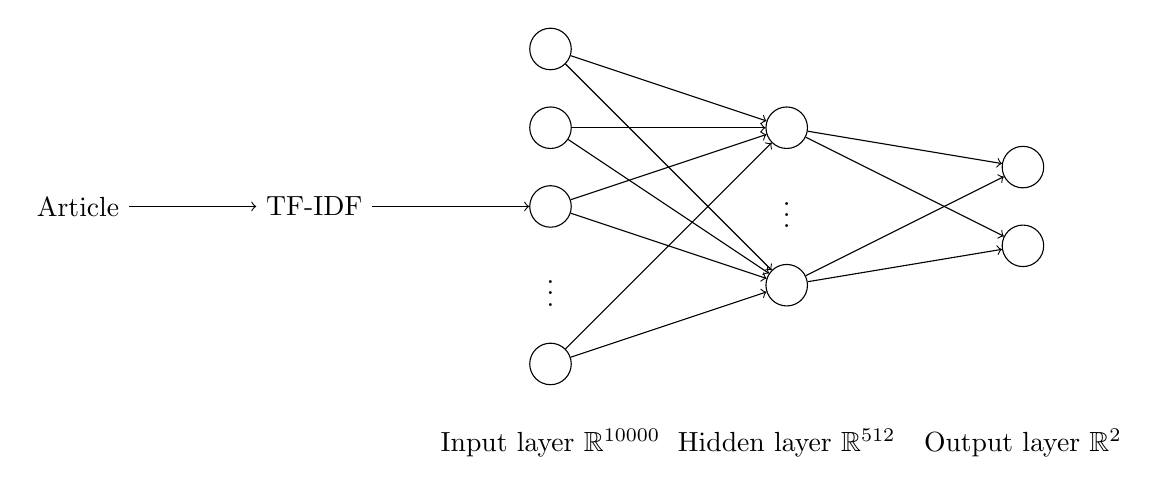
\begin{tikzpicture}
    \tikzset{vertex/.style = {shape=circle,draw,minimum size=1.5em}}

    % Wikipedia Symbol
    \node (wa) at (-6,3) {Article};
    \node (tfidf) at (-3,3) {TF-IDF};

    \draw[->] (wa) -- (tfidf);
        
    % Input Layer
    \node[vertex] (i1) at (0,5) {};
    \node[vertex] (i2) at (0,4) {};
    \node[vertex] (i3) at (0,3) {};
    \node at (0,2) {$\vdots$};
    \node[vertex] (i5) at (0,1) {};
    \node at (0,0) {Input layer $\mathbb{R}^{10000}$};

    \draw[->] (tfidf) -> (i3);
        
    % Hidden Layer
    \node[vertex] (h1) at (3,4) {};
    \node at (3,3) {$\vdots$};
    \node[vertex] (h3) at (3,2) {};
    \node at (3,0) {Hidden layer $\mathbb{R}^{512}$};

    % Arrows between input and hidden layer
    \foreach \j in {1,2,3,5}
        \foreach \k in {1,3}
            \draw[->] (i\j) -- (h\k);
        
    % Output Layer
    \node[vertex] (o1) at (6,3.5) {};
    \node[vertex] (o2) at (6,2.5) {};
    \node at (6,0) {Output layer $\mathbb{R}^{2}$};

    % Arrows between hidden and output layer
    \foreach \j in {1,3}
        \foreach \k in {1,2}
            \draw[->] (h\j) -- (o\k);
\end{tikzpicture}
\end{document}